% IEEE Sensors Journal manuscript v1 (DRN-261027-01). Brief: repo .claude_logs/paper/00_brief.md
% Template: IEEE-JSEN-LaTeX-template-202405 (ieeecolor.cls md5 a08917c6a409f0693d9ac3f1833054b8,
%   jsen.sty md5 f631e3cbadef91d3bbac8bb0024e0448), from IEEE Template Selector, received 2026-10-27.
%   Pristine copies: ../templates/jsen-202405/ (IEEE Access fallback: ../templates/access-20260513/).
\documentclass[journal,twoside,web]{ieeecolor}
\usepackage{jsen}
\usepackage{cite}
\usepackage{amsmath,amssymb,amsfonts}
\usepackage{graphicx}
\usepackage{textcomp}
\usepackage{wrapfig}
\usepackage{booktabs}
\usepackage{multirow}
\usepackage{tikz}
\usetikzlibrary{arrows.meta,calc}
\usepackage[hidelinks]{hyperref}
\definecolor{RED}{rgb}{1,0,0}% running heads are uppercased, which turns `red' into `RED'
\newcommand{\todo}[1]{\textcolor{red}{[TODO: #1]}}
\newcommand{\missing}[1]{\textcolor{blue}{[MISSING: #1]}}
\newcommand{\td}{\textcolor{red}{todo}}% empty table cell, value pending
% table layout: every table uses \tabsetup (same font, same spacing) and spans exactly \columnwidth
\newcommand{\tabsetup}{\footnotesize\setlength{\tabcolsep}{3pt}\renewcommand{\arraystretch}{1.1}}
\newcommand{\tabnote}[1]{\par\vspace{3pt}\parbox{\columnwidth}{\raggedright\scriptsize #1}}
% placeholder frame; the template sets \fboxrule=0pt globally, so restore a visible rule locally
\newcommand{\phbox}[2]{{\setlength{\fboxrule}{0.4pt}\setlength{\fboxsep}{3pt}%
  \fbox{\parbox[c][#1][c]{0.95\linewidth}{\centering\textcolor{red}{todo: #2}}}}}

\markboth{\journalname, VOL. XX, NO. XX, XXXX 2026}
{\todo{Author et al.: short title}}
\definecolor{abstractbg}{rgb}{0.89804,0.94510,0.83137}
\setlength{\fboxrule}{0pt}
\setlength{\fboxsep}{0pt}

\begin{document}
\title{\todo{title}}
\author{\todo{authors and IEEE membership}%
\thanks{\todo{submission date; funding}}%
\thanks{\todo{affiliations and e-mail}}}

\IEEEtitleabstractindextext{%
\fcolorbox{abstractbg}{abstractbg}{%
\begin{minipage}{\textwidth}%
\begin{wrapfigure}[6]{r}{3in}%
{\setlength{\fboxrule}{0.4pt}\fbox{\parbox[c][0.75in][c]{2.9in}{\centering\textcolor{red}{todo: graphical abstract (required by the JSEN template, 3\,in wide)}}}}%
\end{wrapfigure}%
\begin{abstract}
\todo{abstract (write last): one paragraph, 150--250 words, no abbreviations, references, equations or tables (JSEN template rule)}
\end{abstract}

\begin{IEEEkeywords}
% JSEN template: keywords in alphabetical order
Foundation models, missing modality, multimodal semantic segmentation, robustness, sensor fusion
\end{IEEEkeywords}

\end{minipage}}}

\maketitle

\section{Introduction}\label{sec:intro}
\todo{0.8 page: problem, two tracks (accuracy vs. missing-sensor robustness), three contributions}

\section{Related Work}\label{sec:related}
\todo{0.6 page: all-modality fusion; missing-modality robustness; frozen foundation-model adaptation}

\section{Sensors, Benchmarks, and Protocol}\label{sec:sensors}
\todo{0.5 page: sensor physics and failure modes; DELIVER/MUSES/MCubeS; evaluation protocol}

\section{Method}\label{sec:method}
\todo{1.5 pages: architecture figure, two-pass training with teacher distillation, high-resolution path}

% Fig. 1 source: artifact https://claude.ai/artifact/Am5i5hF7CuPQCRuJWibNwc (2026-10-25), redraw as vector (TikZ or PDF).
\begin{figure*}[t]
\centering
\resizebox{\textwidth}{!}{% Fig. 1 — architecture overview (draft drawn in TikZ; redraw guide: ../notes/figure_guide.md).
% Colours: carbon@11.84.0 (labdesign build/py/carbon_palette.py). Sensor colours = CATEGORICAL[0..3].
% Thumbnails: figures/fig1_thumbs/ (make with ../figures/src/make_arch_thumbs.py).
% Coordinates in cm; drawing spans x = 0..18.1 (\textwidth = 18.2 cm). Layout rule: every label
% sits at least 1.5 mm inside its box, and no label crosses a line.
\definecolor{cRGB}{HTML}{6929C4}   % cat-1
\definecolor{cDep}{HTML}{1192E8}   % cat-2
\definecolor{cEvt}{HTML}{005D5D}   % cat-3
\definecolor{cLid}{HTML}{9F1853}   % cat-4
\definecolor{acc}{HTML}{0F62FE}    % accent: trained by us
\definecolor{ink}{HTML}{161616}    % fg
\definecolor{mut}{HTML}{525252}    % fg-muted
\definecolor{bd}{HTML}{C6C6C6}     % border
\definecolor{sf}{HTML}{F4F4F4}     % surface
\definecolor{g20}{HTML}{E0E0E0}    % gray-20
\begin{tikzpicture}[
  x=1cm, y=1cm, font=\sffamily\fontsize{6.5}{7.5}\selectfont, line cap=round, line join=round,
  >={Stealth[length=1.6mm, width=1.2mm]},
  flow/.style={->, draw=mut, line width=0.45pt},
  tflow/.style={->, draw=acc, line width=0.6pt},
  frozen/.style={draw=mut, dash pattern=on 1.6pt off 1.2pt, line width=0.45pt, fill=sf},
  trained/.style={draw=acc, line width=0.7pt, fill=white},
  plain/.style={draw=mut, line width=0.45pt, fill=white},
  ttl/.style={font=\sffamily\bfseries\fontsize{6.8}{8}\selectfont, text=ink},
  sub/.style={text=mut, font=\sffamily\fontsize{5.6}{6.6}\selectfont},
  plab/.style={font=\sffamily\bfseries\fontsize{8}{9}\selectfont, text=ink, anchor=west},
  plus/.style={circle, inner sep=0pt, minimum size=2.6mm, fill=white},
]
% ======================= (a) inference =======================
\node[plab] at (0.0,6.75) {(a)};
\node[ttl, anchor=west] at (0.5,6.75) {Inference: one frozen backbone, sensor-specific adapters, symmetric fusion};

% --- sensor thumbnails ---
\foreach \s/\f/\c/\yy in {RGB/rgb/cRGB/5.15, Depth/depth/cDep/3.9, Event/event/cEvt/2.65, LiDAR/lidar/cLid/1.4}{
  \node[inner sep=0pt] (in\s) at (0.9,\yy) {\includegraphics[width=1.05cm]{figures/fig1_thumbs/\f.png}};
  \draw[\c, line width=0.9pt] (in\s.south west) rectangle (in\s.north east);
  \node[anchor=south, rotate=90, text=\c, font=\sffamily\bfseries\fontsize{6}{7}\selectfont, inner sep=2pt] at (in\s.west) {\s};
}

% --- frozen backbone, one lane per sensor ---
\draw[frozen, rounded corners=1.5pt] (1.8,0.85) rectangle (5.0,6.15);
\node[ttl, anchor=north west] at (1.92,6.02) {DINOv3-L};
\node[sub, anchor=north east] at (4.88,6.0) {frozen, shared};
\node[sub, anchor=east] at (2.62,5.52) {tap};
\foreach \t/\xx in {6/3.25, 12/3.77, 18/4.29, 24/4.81}{ \node[sub] at (\xx,5.52) {\t}; }
\foreach \s/\c/\yy in {RGB/cRGB/5.15, Depth/cDep/3.9, Event/cEvt/2.65, LiDAR/cLid/1.4}{
  \draw[draw=\c, fill=\c!14, line width=0.6pt, rounded corners=0.8pt] (1.97,\yy-0.19) rectangle (2.62,\yy+0.19);
  \node[text=\c, font=\sffamily\bfseries\fontsize{5.2}{6}\selectfont, inner sep=0pt] at (2.295,\yy) {LoRA};
  \foreach \k in {0,...,3}{
    \draw[draw=bd, fill=g20, line width=0.35pt] (2.82+0.52*\k,\yy-0.16) rectangle (3.18+0.52*\k,\yy+0.16);
    \fill[\c] (3.25+0.52*\k,\yy) circle (0.045);
  }
  \draw[flow] (in\s.east) -- (1.97,\yy);
}

% --- per-sensor token sets ---
\node[sub] at (5.5,6.0) {tokens};
\foreach \s/\c/\yy in {RGB/cRGB/5.15, Depth/cDep/3.9, Event/cEvt/2.65, LiDAR/cLid/1.4}{
  \foreach \k in {3,2,1,0}{
    \draw[draw=\c, fill=\c!20, line width=0.4pt] (5.25+0.06*\k,\yy-0.17+0.06*\k) rectangle +(0.3,0.3);
  }
  \coordinate (tok\s) at (5.8,\yy+0.05);
}

% --- cross-modal attention (trained) ---
\draw[trained, rounded corners=1.5pt] (6.2,1.3) rectangle (8.4,5.65);
\node[ttl, align=center] at (7.3,5.12) {Cross-modal\\attention};
\coordinate (K) at (7.3,3.55);
\foreach \s/\a in {RGB/135, Depth/45, Event/-45, LiDAR/-135}{ \coordinate (n\s) at ($(K)+(\a:0.68)$); }
\foreach \p/\q in {RGB/Depth, RGB/Event, RGB/LiDAR, Depth/Event, Depth/LiDAR, Event/LiDAR}{
  \draw[<->, draw=mut!70, line width=0.4pt, >={Stealth[length=1.1mm,width=0.9mm]}, shorten <=1.5mm, shorten >=1.5mm] (n\p) -- (n\q);
}
\foreach \s/\c in {RGB/cRGB, Depth/cDep, Event/cEvt, LiDAR/cLid}{ \fill[\c] (n\s) circle (0.1); }
\node[sub, align=center] at (7.3,1.9) {each sensor attends\\to the others\\2 layers, no gate};
\foreach \s/\yy in {RGB/4.85, Depth/3.95, Event/3.05, LiDAR/2.2}{
  \draw[flow] (tok\s) to[out=0, in=180] (6.2,\yy);
}

% --- SimpleFPN (conventional) ---
\draw[plain, draw=bd, rounded corners=1.5pt] (8.68,1.7) rectangle (10.15,5.65);
\node[ttl] at (9.45,5.38) {SimpleFPN};
\foreach \lab/\w/\yy in {{1/32}/0.32/4.75, {1/16}/0.44/4.05, {1/8}/0.58/3.2, {1/4}/0.76/2.2}{
  \draw[plain] (9.6-\w/2,\yy-\w/2) rectangle (9.6+\w/2,\yy+\w/2);
  \node[sub, anchor=east] at (9.6-\w/2-0.06,\yy) {\lab};
}
\draw[flow] (8.4,3.2) -- (8.68,3.2);
\node[plus, draw=mut, line width=0.45pt] (sum) at (9.6,1.05) {};
\draw[mut, line width=0.45pt] (sum.north) -- (sum.south) (sum.west) -- (sum.east);
\draw[flow] (sum) -- (9.6,1.82);
\node[sub, anchor=west] at (9.78,1.05) {sum per level};

% --- high-resolution path (adopted from the DINOv3 adapter) ---
\draw[flow] (inLiDAR.south) -- (0.9,0.35) -- (2.05,0.35);
\node[sub, anchor=north] at (1.47,0.3) {full-res. input};
\draw[plain, rounded corners=1.2pt] (2.05,0.12) rectangle (3.45,0.58);
\node[text=ink] at (2.75,0.35) {conv stem};
\draw[flow] (3.45,0.35) -- (3.8,0.35);
\draw[plain, rounded corners=1.2pt] (3.8,0.12) rectangle (6.75,0.58);
\node[text=ink] at (5.275,0.35) {deformable extractor ($\times$4)};
\draw[->, draw=mut, line width=0.45pt, dash pattern=on 1.4pt off 1pt] (4.35,0.85) -- (4.35,0.58);
\node[sub, anchor=west] at (4.42,0.72) {samples tap tokens};
\draw[flow] (6.75,0.35) -| (sum.south);
\node[sub, anchor=south] at (8.1,0.38) {high-resolution path};

% --- heads (trained) ---
\draw[flow] (10.15,3.2) -- (10.3,3.2) |- (10.5,4.75);
\draw[flow] (10.3,3.35) -- (10.5,3.35);
\draw[trained, rounded corners=1.2pt] (10.5,4.4) rectangle (11.95,5.1);
\node[ttl] at (11.225,4.87) {Dense head};
\node[sub] at (11.225,4.6) {per-pixel};
\draw[trained, rounded corners=1.2pt] (10.5,2.75) rectangle (11.95,3.95);
\node[ttl] at (11.225,3.7) {Query head};
\foreach \k in {0,...,7}{ \fill[acc!55] (10.805+0.12*\k,3.36) circle (0.035); }
\node[sub] at (11.225,3.03) {100 queries};
\node[plus, draw=acc, line width=0.6pt] (arb) at (12.35,3.35) {};
\draw[acc, line width=0.6pt] (arb.north) -- (arb.south) (arb.west) -- (arb.east);
\draw[tflow] (11.95,4.75) -| (12.75,3.35) -- (arb.east);
\draw[tflow] (11.95,3.35) -- (arb.west);
\node[sub, anchor=north west] at (12.45,3.2) {arbiter};
\node[inner sep=0pt] (pred) at (12.35,1.45) {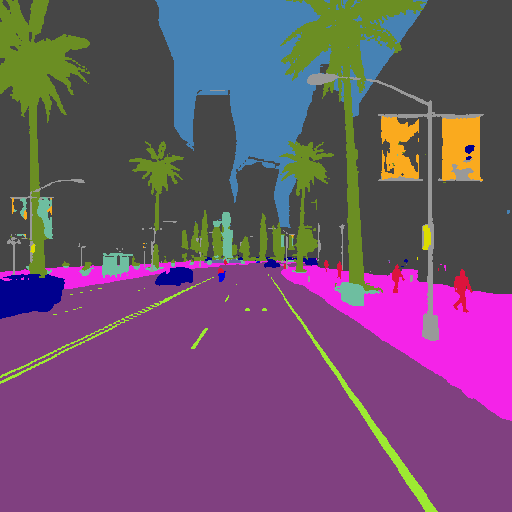
\includegraphics[width=1.05cm]{figures/fig1_thumbs/pred.png}};
\draw[ink, line width=0.5pt] (pred.south west) rectangle (pred.north east);
\draw[tflow] (arb.south) -- (pred.north);
\node[sub, anchor=north] at (pred.south) {prediction};

% ======================= (b) training =======================
\draw[bd, line width=0.4pt] (13.2,0.05) -- (13.2,6.6);
\node[plab] at (13.35,6.75) {(b)};
\node[ttl, anchor=west] at (13.85,6.75) {Training: clean and degraded passes};

\node[inner sep=0pt] (cl) at (14.1,4.9) {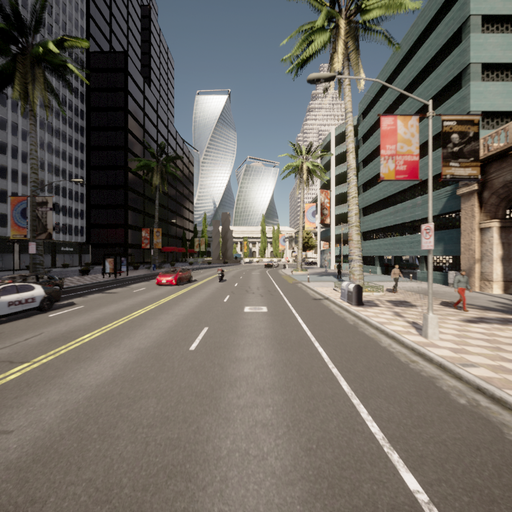
\includegraphics[width=0.95cm]{figures/fig1_thumbs/rgb.png}};
\node[sub, anchor=north] at (cl.south) {clean};
% degraded RGB in front of a dropped sensor
\draw[draw=mut, fill=white, line width=0.4pt] (14.1-0.475+0.15,2.8-0.475-0.15) rectangle (14.1+0.475+0.15,2.8+0.475-0.15);
\draw[mut, line width=0.35pt] (14.1-0.475+0.15,2.8-0.475-0.15) -- (14.1+0.475+0.15,2.8+0.475-0.15);
\node[inner sep=0pt] (dg) at (14.1,2.8) {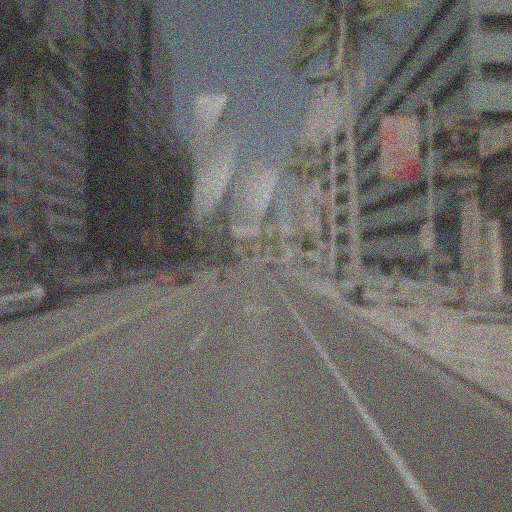
\includegraphics[width=0.95cm]{figures/fig1_thumbs/rgb_degraded.png}};
\node[sub, anchor=north, align=center] at (14.2,2.12) {degraded\\(noise, blur,\\dropout)};

\draw[trained, rounded corners=1.5pt] (14.95,2.3) rectangle (16.45,5.4);
\node[ttl] at (15.7,4.05) {Model (a)};
\node[sub, align=center] at (15.7,3.62) {same\\weights};
\draw[flow] (cl.east) -- (14.95,4.9);
\draw[flow] (dg.east) ++(0.15,0) -- (14.95,2.8);

\draw[frozen, rounded corners=1.5pt] (14.95,0.3) rectangle (16.45,1.5);
\node[ttl] at (15.7,1.2) {Teacher};
\node[sub, align=center] at (15.7,0.77) {frozen,\\clean-trained};
\draw[flow] (cl.west) -- (13.38,4.9) |- (14.95,0.9);

\node[anchor=west, text=ink, inner sep=1pt] (ce1) at (16.85,4.9) {$\mathcal{L}_{\mathrm{CE}}$};
\node[anchor=west, text=ink, inner sep=1pt] (ce2) at (16.85,3.2) {$\mathcal{L}_{\mathrm{CE}}$};
\node[anchor=west, text=acc, inner sep=1pt] (kd) at (16.85,2.4) {$\mathcal{L}_{\mathrm{KD}}$};
\draw[flow] (16.45,4.9) -- (ce1.west);
\draw[flow] (16.45,2.8) -- (16.65,2.8) |- (ce2.west);
\draw[flow] (16.65,2.8) |- (kd.west);
\draw[->, draw=acc, line width=0.55pt, dash pattern=on 1.4pt off 1pt] (16.45,0.9) -| (kd.south);
\node[sub, anchor=west, align=left] at (17.25,1.3) {soft\\targets\\$T{=}2$};
\end{tikzpicture}
}
\caption{Overview. (a) Each sensor passes through the same frozen DINOv3-L with its own LoRA adapter; tokens from four depths are fused by symmetric cross-modal attention, decoded by a SimpleFPN augmented with a high-resolution path, and classified by a dense head and a query head combined by an arbiter. (b) Every batch is used twice: a clean pass and a synthetically degraded pass, the latter also distilled from a frozen teacher trained on clean data. Blue outlines mark trained components; dashed boxes are frozen. \todo{draft drawn by the paper session; redraw per notes/figure\_guide.md}}
\label{fig:arch}
\end{figure*}

\section{Experiments}\label{sec:exp}
\todo{2.5 pages: implementation details (frozen DINOv3-L, LoRA r8, 40-epoch schedule, val-best checkpoint, legal v2 at 1024), then Tables 1--7}

% Layout rule (user 2026-10-27): no \resizebox on tables. Every table uses \tabsetup and
% tabular* at \columnwidth, so all tables share one font size and none overflows the column.

% ---------------------------------------------------------------------------
% Table 1. DELIVER, all four sensors.
% Baselines: only the test-unified cluster (DGFusion protocol, "mIoU-test").
%   Do NOT mix with the high cluster (CMNeXt 66.30 / MemorySAM 65.38).
%   Candidate values for todo cells are in repo research/novelty-and-related-work.md:78-83
%   (secondary copy) -> must be taken from each original paper table, cite table+page.
% Ours: experiments/headline.yaml benchmarks.deliver.ours[0] (A2, 3 seeds, legal v2, test@1024).
%   val 3-seed mean is not recorded in headline.yaml (only seed903 69.86) -> todo.
% ---------------------------------------------------------------------------
\begin{table}[t]
\caption{DELIVER (RGB, depth, event, LiDAR), mIoU (\%).}
\label{tab:deliver}
\centering\tabsetup
\begin{tabular*}{\columnwidth}{@{\extracolsep{\fill}}lllcc@{}}
\toprule
Method & Backbone & Sensors & val & test \\
\midrule
CMNeXt~\td & \td & RGB-D-E-L & \td & \td \\
StitchFusion~\td & \td & RGB-D-E-L & \td & \td \\
GeminiFusion~\td & \td & RGB-D-E-L & \td & \td \\
CAFuser~\td & \td & RGB-D-E-L & \td & \td \\
CAFuser-CAA~\td & \td & RGB-D-E-L & 68.79 & \td \\
DGFusion~\td & Swin-T & RGB-D-E-L & \td & 56.71 \\
\midrule
\multicolumn{5}{@{}l}{\emph{Fewer sensors (secondary comparison)}} \\
MM SAM-adapter~\td & \td & RGB-D & 69.60 & 57.35 \\
\midrule
Ours (3-seed mean) & DINOv3-L & RGB-D-E-L & \td & 57.74 \\
Ours (best seed) & DINOv3-L & RGB-D-E-L & \td & 58.61 \\
\bottomrule
\end{tabular*}
\tabnote{\textcolor{red}{todo: original table/page per baseline; protocol (val-best checkpoint, 1024, nearest-exact label resampling); DINOv3-L is frozen.}}
\end{table}

% ---------------------------------------------------------------------------
% Table 2. MUSES, four sensors (RGB, event, LiDAR, radar). Only the 4-sensor A2 model
%   (user 2026-09-29; 3-sensor numbers 79.788 etc. are not used).
% Ours: DRN-261019-02 (queued) -> todo. Baselines: headline.yaml benchmarks.muses.
% ---------------------------------------------------------------------------
\begin{table}[t]
\caption{MUSES, official evaluation, mIoU (\%).}
\label{tab:muses}
\centering\tabsetup
\begin{tabular*}{\columnwidth}{@{\extracolsep{\fill}}lllcc@{}}
\toprule
Method & Backbone & Sensors & val & test \\
\midrule
CAFuser~\td & \td & \td & \td & \td \\
DGFusion~\td & \td & \td & \td & 79.5 \\
\midrule
\multicolumn{5}{@{}l}{\emph{Camera only or fewer sensors (secondary comparison)}} \\
GtA~\td & \td & RGB & \td & 82.39 \\
MM SAM-adapter~\td & \td & RGB-L & \td & 81.07 \\
\midrule
Ours & DINOv3-L & RGB-E-L-R & \td & \td \\
\bottomrule
\end{tabular*}
\end{table}

% ---------------------------------------------------------------------------
% Table 3. MCubeS (RGB, AoLP, DoLP, NIR). Ours: DRN-261017-02 (A2 transfer, 2 seeds) -> todo.
%   58.07 in headline.yaml is the previous generation (P39.1 recipe), not the paper model.
% ---------------------------------------------------------------------------
\begin{table}[t]
\caption{MCubeS (RGB, AoLP, DoLP, NIR), test mIoU (\%).}
\label{tab:mcubes}
\centering\tabsetup
\begin{tabular*}{\columnwidth}{@{\extracolsep{\fill}}llc@{}}
\toprule
Method & Backbone & test \\
\midrule
Mul-VMamba~\td & \td & 54.65 \\
StitchFusion~\td & \td & 55.9 \\
\midrule
Ours & DINOv3-L & \td \\
\bottomrule
\end{tabular*}
\end{table}

% ---------------------------------------------------------------------------
% Table 4. Missing and degraded sensors on DELIVER.
% (a) Benchmark family (2503.18445 definition: normalize then zero-fill), val.
%     Ours: tasks/DRN-261019-03/analysis.md (A2 3 seeds, mm_eval_v2): EMM15 57.85,
%     RMM15 r.25/.5/.75 65.53/63.35/61.28. RMMSS EMM 49.93: same doc / headline.yaml note.
% (b) Same protocol, our measurement on test (61 cases, 1897 images):
%     DGFusion (a) official weights / (b) degradation retrained: experiments/judgment-ledger.md
%       2026-10-01 row (DRN-260930-02). CAFuser (b): status/current.md (4) "CAFuser (b) 10-04".
%     "w/o two-pass" = E1 40ep screen 3 seeds, EMM 40.01: ledger 2026-10-01 row.
%     "w/o high-res" = Q2 3 seeds, "Ours" = A2 3 seeds: tasks/DRN-261019-03/analysis.md
%       (Q2 NM is 2 seeds for s902/s903 plus s821 where available; see that table).
%     Depth/RGB partial-drop columns omitted: Q2 values disagree between ledger 10-01 (3 seeds:
%     0.98/2.04/2.64) and DRN-261019-03 (2 seeds: 0.47/1.05/1.36) -> resolve before use.
% Families that skip missing inputs (AnySeg, RMMSS, RobustSeg 1a, FuseAdapt) are not mixed here.
% ---------------------------------------------------------------------------
\begin{table}[t]
\caption{Robustness to missing and degraded sensors on DELIVER, mIoU (\%).}
\label{tab:robust}
\centering\tabsetup
\begin{tabular*}{\columnwidth}{@{\extracolsep{\fill}}lccccc@{}}
\toprule
\multicolumn{6}{@{}l}{\emph{(a) Public missing-modality benchmark, val}} \\
Method & EMM & RMM .25 & RMM .50 & RMM .75 & \\
\midrule
RMMSS~\td & 49.93 & \td & \td & \td & \\
Ours (3 seeds) & 57.85 & 65.53 & 63.35 & 61.28 & \\
\midrule
\multicolumn{6}{@{}l}{\emph{(b) Same protocol for all models, test}} \\
Method & Clean & EMM & S\&P .05 & S\&P .10 & S\&P .20 \\
\midrule
DGFusion (official) & 55.68 & 31.53 & 37.97 & 16.71 & 5.52 \\
DGFusion (retrained$^{\dagger}$) & 54.77 & 45.52 & 48.89 & 40.51 & 23.34 \\
CAFuser (retrained$^{\dagger}$) & 55.79 & 46.50 & \td & \td & \td \\
Ours w/o two-pass & \td & 40.01 & \td & \td & \td \\
Ours w/o high-res & 56.59 & 48.06 & 53.25 & 51.64 & 48.79 \\
Ours & 57.74 & 48.66 & 53.11 & 51.36 & 47.85 \\
\bottomrule
\end{tabular*}
\tabnote{$^{\dagger}$Retrained with the same synthetic degradation. Ours: mean of 3 seeds; baselines: single runs.
\textcolor{red}{todo: define EMM (mean over 15 sensor subsets), RMM (random drop ratio), S\&P noise.}}
\end{table}

% ---------------------------------------------------------------------------
% Fig. robust (data plot). Source numbers and provenance: figures/src/make_data_figs.py (fig_robust).
% ---------------------------------------------------------------------------
\begin{figure}[t]
\centering
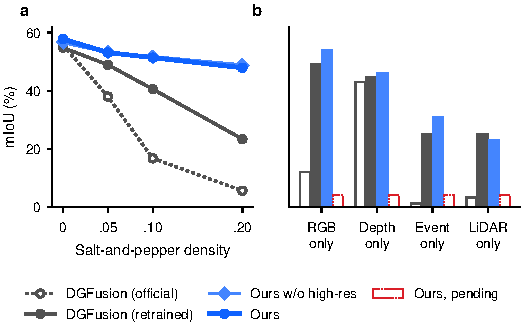
\includegraphics[width=\columnwidth]{figures/fig_robust.pdf}
\caption{Robustness on DELIVER test under one protocol. (a) Salt-and-pepper noise applied to every sensor. (b) Only one sensor available (the other three zero-filled). Ours: mean of three seeds; DGFusion: single runs, official weights or retrained with the same synthetic degradation. \todo{(b) full-model values pending.}}
\label{fig:robust}
\end{figure}

% Fig. sensor-failure scenarios (main qualitative figure). Needs per-image predictions of
% DGFusion (official), DGFusion/CAFuser (retrained) and ours under missing/noisy sensors
% -> analysis request inbox 20261027-182054 item 2.
\begin{figure*}[t]
\centering
\phbox{5.2cm}{Fig.~3 when a sensor fails: rows = depth missing / RGB missing / LiDAR+event missing / RGB with heavy noise; columns = affected input, ground truth, DGFusion (official), DGFusion (retrained), CAFuser (retrained), ours; error pixels in one colour}
\caption{\todo{caption; state the scene-selection rule (top differences between ours and the best baseline, one scene per condition, no repeated map)}}
\label{fig:failure_scenarios}
\end{figure*}

% Fig. adverse conditions with all sensors present, DELIVER (synthetic) + MUSES (real).
% DELIVER dumps exist: NAS analysis_logs/native_axis_baseline_20261016/{dgfusion,cafuserb}_test1024,
% a2_test1024_dump_20261016/s821 -> analysis request inbox 20261027-182054 item 1. MUSES: item 3.
\begin{figure*}[t]
\centering
\phbox{4.6cm}{Fig.~4 adverse conditions, all sensors present: DELIVER night / fog / rain / low exposure and MUSES real night / snow / fog; columns = RGB, ground truth, DGFusion, CAFuser, ours; zoomed crops where the baselines miss objects}
\caption{\todo{caption; state the scene-selection rule}}
\label{fig:adverse}
\end{figure*}

% ---------------------------------------------------------------------------
% Table 5. Clean mIoU per condition on DELIVER test (new 2026-10-28, user: 10-page budget).
% Source: to be computed by analysis from the same dumps as Fig. adverse (inbox addendum).
% ---------------------------------------------------------------------------
\begin{table}[t]
\caption{DELIVER test mIoU (\%) per condition, all sensors present.}
\label{tab:condition}
\centering\tabsetup
\begin{tabular*}{\columnwidth}{@{\extracolsep{\fill}}lccccccc@{}}
\toprule
Model & Sun & Cloud & Rain & Fog & Night & Low exp. & All \\
\midrule
DGFusion (official) & \td & \td & \td & \td & \td & \td & 55.68 \\
DGFusion (retrained$^{\dagger}$) & \td & \td & \td & \td & \td & \td & 54.77 \\
CAFuser (retrained$^{\dagger}$) & \td & \td & \td & \td & \td & \td & 55.79 \\
Ours w/o high-res & \td & \td & \td & \td & \td & \td & 56.59 \\
Ours & \td & \td & \td & \td & \td & \td & 57.74 \\
\bottomrule
\end{tabular*}
\tabnote{$^{\dagger}$Retrained with synthetic degradation. All: same values as Table~\ref{tab:robust}(b) clean column.}
\end{table}

% ---------------------------------------------------------------------------
% Table 6. Ablation on DELIVER test, seed 821, 40 epochs, legal v2.
% RGB-only 55.14 = judgment-ledger 2026-10-28 DRN-261020-08 (adopted as ladder row).
% L1 shared LoRA 58.84, L2 mean fusion 57.76, L4 dense head only 57.89 = judgment-ledger 2026-10-28
%   rows DRN-261020-09/-10/-12 (test@1024 legal v2, seed 821). L2 also removes the trunk expansion
%   (code constraint, ledger note). L5 DRN-261020-13 / L6 -14 evaluating; mean-fusion ladder -07 running.
% mean fusion = DRN-261020-07 (evaluating). E1 screen s821 55.94 = status/current.md (4).
% Q2 s821 57.73 / EMM 48.68 and A2 s821 58.61 / EMM 49.12 = tasks/DRN-261019-03/analysis.md.
% Leave-one-out: L1 DRN-261020-09, L2 -10, L4 -12, L5 -13, L6 -14 (queued). L3 withdrawn.
% ---------------------------------------------------------------------------
\begin{table}[t]
\caption{Ablation on DELIVER test (one seed, 40 epochs), mIoU (\%).}
\label{tab:ablation}
\centering\tabsetup
\begin{tabular*}{\columnwidth}{@{\extracolsep{\fill}}lcc@{}}
\toprule
Configuration & Clean & EMM \\
\midrule
\multicolumn{3}{@{}l}{\emph{Building up}} \\
Frozen DINOv3-L + LoRA, RGB only & 55.14 & -- \\
+ depth, event, LiDAR (mean fusion) & \td & \td \\
+ cross-modal attention, query head & 55.94 & \td \\
+ two-pass training, distillation & 57.73 & 48.68 \\
+ high-res path (full model) & 58.61 & 49.12 \\
\midrule
\multicolumn{3}{@{}l}{\emph{Removing one component from the full model}} \\
$-$ sensor-specific LoRA (one shared) & 58.84 & \td \\
$-$ cross-modal attention (mean fusion)$^{*}$ & 57.76 & \td \\
$-$ query head and arbiter & 57.89 & \td \\
$-$ degradation pass & \td & \td \\
$-$ teacher distillation & \td & \td \\
\bottomrule
\end{tabular*}
\tabnote{$^{*}$Also removes the trunk expansion. \textcolor{red}{todo: EMM column for ablation runs; decision on shared LoRA pending its robustness test.}}
\end{table}

% ---------------------------------------------------------------------------
% Table 7. Cost on DELIVER at 1024, same GPU. DRN-261027-02 (queued) -> all todo.
% ---------------------------------------------------------------------------
\begin{table}[t]
\caption{Computational cost on DELIVER at $1024\times1024$.}
\label{tab:cost}
\centering\tabsetup
\begin{tabular*}{\columnwidth}{@{\extracolsep{\fill}}lccccc@{}}
\toprule
Model & Params & Trainable & GFLOPs & Latency & Memory \\
 & (M) & (M) & & (ms) & (GB) \\
\midrule
DGFusion & \td & \td & \td & \td & \td \\
CAFuser & \td & \td & \td & \td & \td \\
Ours w/o high-res & \td & \td & \td & \td & \td \\
Ours & \td & \td & \td & \td & \td \\
\bottomrule
\end{tabular*}
\end{table}

\section{Analysis}\label{sec:analysis}
\todo{1.5 pages: where the sensor over-reliance comes from, source of the resolution gain, thin objects, failure case, limitations}

% Figure plan: notes/figure_guide.md §2. Qualitative scenes come from recorded dumps only
% (path + md5 in the figure source note) and the selection rule is stated in the caption.

% Fig. dependence (data plot, main evidence for contribution 1).
% Source numbers and provenance: figures/src/make_data_figs.py (fig_dependence).
% Full table: sections/supp_tables.tex (supplementary Table S1).
\begin{figure}[t]
\centering
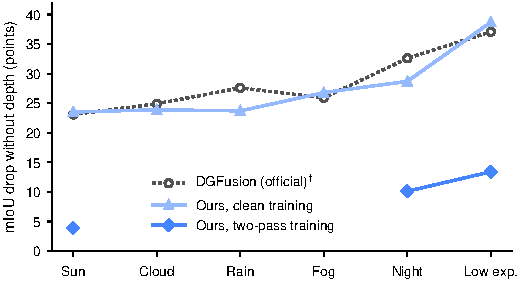
\includegraphics[width=\columnwidth]{figures/fig_dependence.pdf}
\caption{Drop in mIoU when depth is removed, per condition. A model trained only on clean data relies on depth as heavily as DGFusion, whose design adds depth supervision; two-pass training reduces the drop to a third or less with the same architecture. $^{\dagger}$Measured on test; the other curves on val. \todo{re-measure all curves on one split; add the full model and the retrained baselines.}}
\label{fig:dependence}
\end{figure}

% Fig. thin objects. Source: .claude_logs/experiments/analysis/DRN-261018-01/a2_vs_q2_perclass_3seed.csv
% (3 seeds, legal v2 test 1024); plot: figures/src/make_data_figs.py (fig_thin).
\begin{figure}[t]
\centering
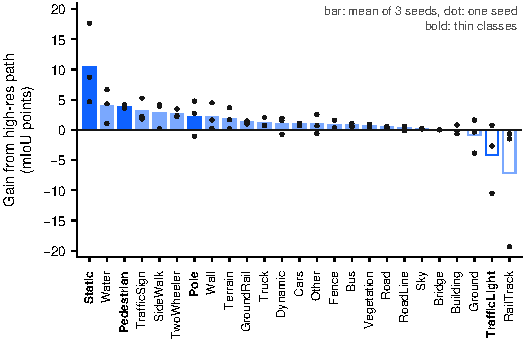
\includegraphics[width=\columnwidth]{figures/fig_thin.pdf}
\caption{Per-class gain of the high-resolution path on DELIVER test, paired by seed (full model minus the same model without the path). Thin classes gain most; TrafficLight and RailTrack lose and vary strongly across seeds (Section~\ref{sec:analysis}). \todo{add zoomed crops of thin objects (Q2 dumps on yeon).}}
\label{fig:thin}
\end{figure}

% Fig. failure case, posters predicted as traffic lights.
% Assets: NAS analysis_logs/a2_tl_fp_scenes_20261022 (4 scenes, README.md has the selection rule).
\begin{figure}[t]
\centering
\phbox{4.2cm}{limitation: posters and signs predicted as traffic light (2 of the 4 recorded scenes; RGB, ground truth, ours, error map)}
\caption{\todo{caption; selection rule from the scene README}}
\label{fig:failure}
\end{figure}

\section{Conclusion}\label{sec:conclusion}
\todo{0.3 page}


% bibliography enabled once sections contain \cite (empty thebibliography breaks the build)
%\bibliographystyle{IEEEtran}
%\bibliography{IEEEabrv,references}

% Author biographies with photos (template includes them; required for IEEE Access).
% \begin{IEEEbiography}[{\includegraphics[width=1in,height=1.25in,clip,keepaspectratio]{a1.png}}]{Name} ...\end{IEEEbiography}
\end{document}
